\documentclass[12pt,a4paper]{article}

\usepackage{fullpage}
\usepackage[utf8]{inputenc}
\usepackage[english]{babel}
\usepackage[dvipsnames]{xcolor}
\usepackage{amssymb, amsmath}
\usepackage{parskip, enumitem}
\usepackage{graphicx}
\usepackage{hyperref}
\hypersetup{colorlinks, linkcolor={red!50!black}, citecolor={blue!50!black}, urlcolor={blue!80!black}}

\DeclareGraphicsExtensions{.eps, .png, .gif, .pdf, .jpg}
\graphicspath{{../v01/OUTPUT/}}

\renewcommand{\vec}[1]{\mathbf{#1}}
\newcommand{\from}{\colon}
\newcommand{\IR}{\mathbb{R}}
\newcommand{\IN}{\mathbb{N}}
\newcommand{\norm}[1]{\left\|#1\right\|}

\begin{document}
    
    %%%%%%%%%%%%%%%%%%%%%%%%%%%%%%%%%%%%%%%%%%%%%%%%%%
    Dida hwk report
    \hfill
    R.A., \today
    %%%%%%%%%%%%%%%%%%%%%%%%%%%%%%%%%%%%%%%%%%%%%%%%%%
    
    %%%%%%%%%%%%%%%%%%%%%%%%%%%%%%%%%%%%%%%%%%%%%%%%%%
    \subsubsection*{Attribution}
    %%%%%%%%%%%%%%%%%%%%%%%%%%%%%%%%%%%%%%%%%%%%%%%%%%
    
    The satellite images shown below are from Mapbox
    in the vicinity of Rosdorf/G\"ottingen, Germany,
    obtained as described in 
    R.A., \href{https://medium.com/@busybus/rendered-maps-with-python-ffba4b34101c}{``Rendered maps with Python''} on Medium.
    %
    The grayscale label images are constructed 
    from OpenStreetMap data,
    downloaded (2019-10-16) from the Overpass API
    filtered by \texttt{building=*}
    via 
    the JOSM desktop app.
    
    %%%%%%%%%%%%%%%%%%%%%%%%%%%%%%%%%%%%%%%%%%%%%%%%%%
    \subsubsection*{Problem statement \& datasets}
    %%%%%%%%%%%%%%%%%%%%%%%%%%%%%%%%%%%%%%%%%%%%%%%%%%
    
    The task is to label buildings in satellite images of 
    rural areas as follows:
    
    \begin{center}
        \begin{minipage}{0.3\textwidth}
            \centering given 
            \\
            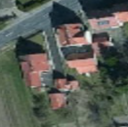
\includegraphics[width=\textwidth]{from_josm/rosdorf/examples/image_3DJFEM}
        \end{minipage}
        %
        \qquad
        %
        \begin{minipage}{0.3\textwidth}
            \centering wanted 
            \\
            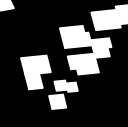
\includegraphics[width=\textwidth]{from_josm/rosdorf/examples/label_3DJFEM}
        \end{minipage}
    \end{center}
    
    The ``Dida'' dataset contains 
    %
    \begin{itemize}
    \item 
        30 satellite (or similar) images of size $256 \times 256 \times \text{RGBA}$,
        and
    \item
        25 grayscale label images of unknown origin.
        %
        One duplicate mislabel is omitted.
    \end{itemize}
    %
    The the alpha channel is  
    presumably used to indicate missing or sensitive data.
    
    %
    
    More specifically now, the aim is to construct a neural network 
    image segmentation predictor
    and
    use it on the 5 unlabeled satellite images
    of the ``Dida'' dataset.
    
    %
    
    The ``Mapbox/OSM'' dataset, obtained as described in the beginning,
    contains 359 RGB images of size $128 \times 128$
    with the corresponding grayscale label images. 
    %
    While Mapbox satellite images are well-aligned,
    they are outdated compared to OpenStreetMap building annotations.
    %
    The images/label pairs have been hand-selected 
    from a somewhat larger pool
    to make sure they are still compatible,
    i.e.~refer to the same (on-the-)ground truth.
    
    %
    
    The datasets are 
    downscaled to $128 \times 128$
    and
    augmented $8$-fold by 
    rotation and mirroring.

    
    %%%%%%%%%%%%%%%%%%%%%%%%%%%%%%%%%%%%%%%%%%%%%%%%%%
    \subsubsection*{Neural net architecture}
    %%%%%%%%%%%%%%%%%%%%%%%%%%%%%%%%%%%%%%%%%%%%%%%%%%
    
    Our neural network
    is essentially 
    the MobileNetV2-derived
    encoder-decoder ``U-Net''
    from the TensorFlow2 image segmentation tutorial
    \begin{quote}
        \href{https://www.tensorflow.org/tutorials/images/segmentation}{https://www.tensorflow.org/tutorials/images/segmentation}.
    \end{quote}
    %
    %
    The predictor is 
    constructed 
    by tapping into several 
    progressively narrow layers 
    of the pretrained and frozen
    image classifier MobileNetV2 (encoder)
    and
    by combining their activations/outputs using 
    trainable 
    convolutional
    upsampling layers (decoder).
    %
    %
    The MobileNetV2 encoder 
    takes a $128 \times 128 \times \text{RGB}$ image;
    therefore,
    the alpha channel is split off
    before the ``U-Net''
    and 
    concatenated again with its output.
    %
    The result is then passed through another
    convolution layer with two filters
    with a $128 \times 128 \times 2$ output.
    %
    %
    The channel dimension is 
    interpreted as the predicted pixel label/class confidence
    (non-building vs.~building).
    %
    %
    This is a departure from the tutorial
    that also includes the ``object boundary'' class.
    %
    %
    A graphical summary is shown in Fig.~\ref{f:model}.
    
    
    

    %%%%%%%%%%%%%%%%%%%%%%%%%%%%%%%%%%%%%%%%%%%%%%%%%%
    \subsubsection*{Results}
    %%%%%%%%%%%%%%%%%%%%%%%%%%%%%%%%%%%%%%%%%%%%%%%%%%
    
    We train the same model with the Adam optimizer on 
    the pixelwise cross-entropy loss 
    for 33 epochs,
    setting apart 20\% of data for validation,
    either 
    \begin{itemize}
    \item 
        only on the ``Dida'' dataset (Scenario I), or
    \item
        on both ``Dida'' and ``Mapbox/JOSM'' datasets (Scenario II).
    \end{itemize}
    
    The results are shown in Fig.~\ref{f:loss} and \ref{f:labels}.
    
    
    \begin{figure}[p]
        \centering
        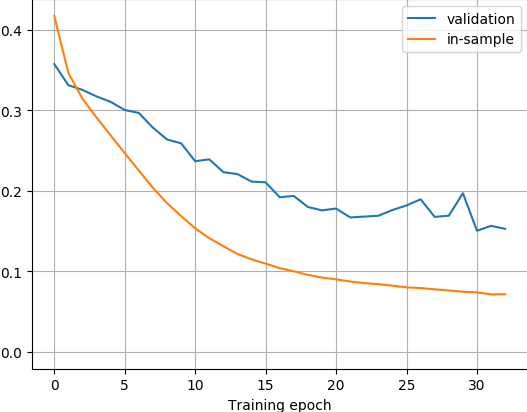
\includegraphics[width=0.48\textwidth]{images/data_onlydida/last_history}
        \hfill
        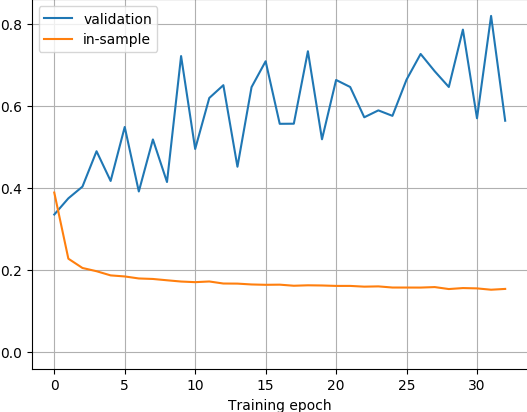
\includegraphics[width=0.48\textwidth]{images/data_withjosm/last_history}
        
        \caption{Cross-entropy loss, scenario I (left) and II (right).}
        \label{f:loss}
    \end{figure}
    
    
    \begin{figure}[p]
        \centering

        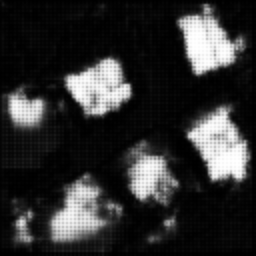
\includegraphics[width=0.19\textwidth]{images/data_onlydida/predictions/535}
        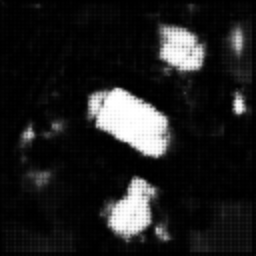
\includegraphics[width=0.19\textwidth]{images/data_onlydida/predictions/537}
        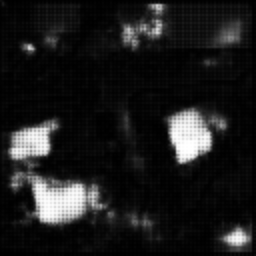
\includegraphics[width=0.19\textwidth]{images/data_onlydida/predictions/539}
        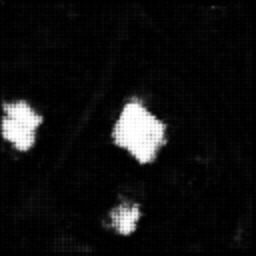
\includegraphics[width=0.19\textwidth]{images/data_onlydida/predictions/551}
        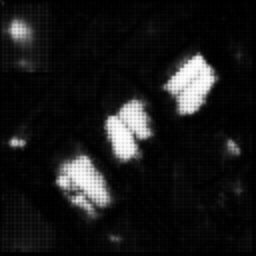
\includegraphics[width=0.19\textwidth]{images/data_onlydida/predictions/553}
        
        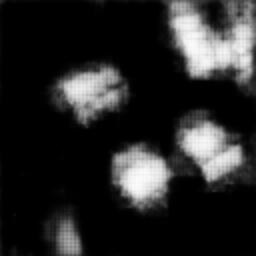
\includegraphics[width=0.19\textwidth]{images/data_withjosm/predictions/535}
        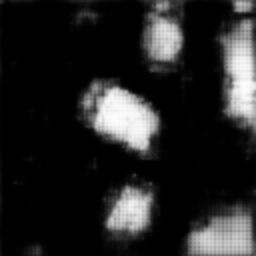
\includegraphics[width=0.19\textwidth]{images/data_withjosm/predictions/537}
        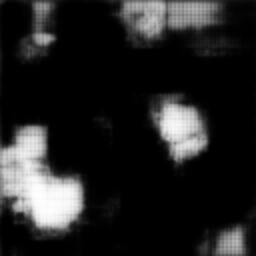
\includegraphics[width=0.19\textwidth]{images/data_withjosm/predictions/539}
        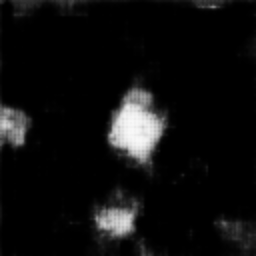
\includegraphics[width=0.19\textwidth]{images/data_withjosm/predictions/551}
        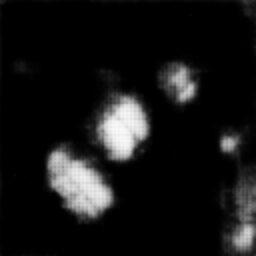
\includegraphics[width=0.19\textwidth]{images/data_withjosm/predictions/553}
        
        \caption{Missing Dida labels, scenario I (top) and II (bottom).}
        \label{f:labels}
    \end{figure}

    
    
    \begin{figure}[p]
        \centering
        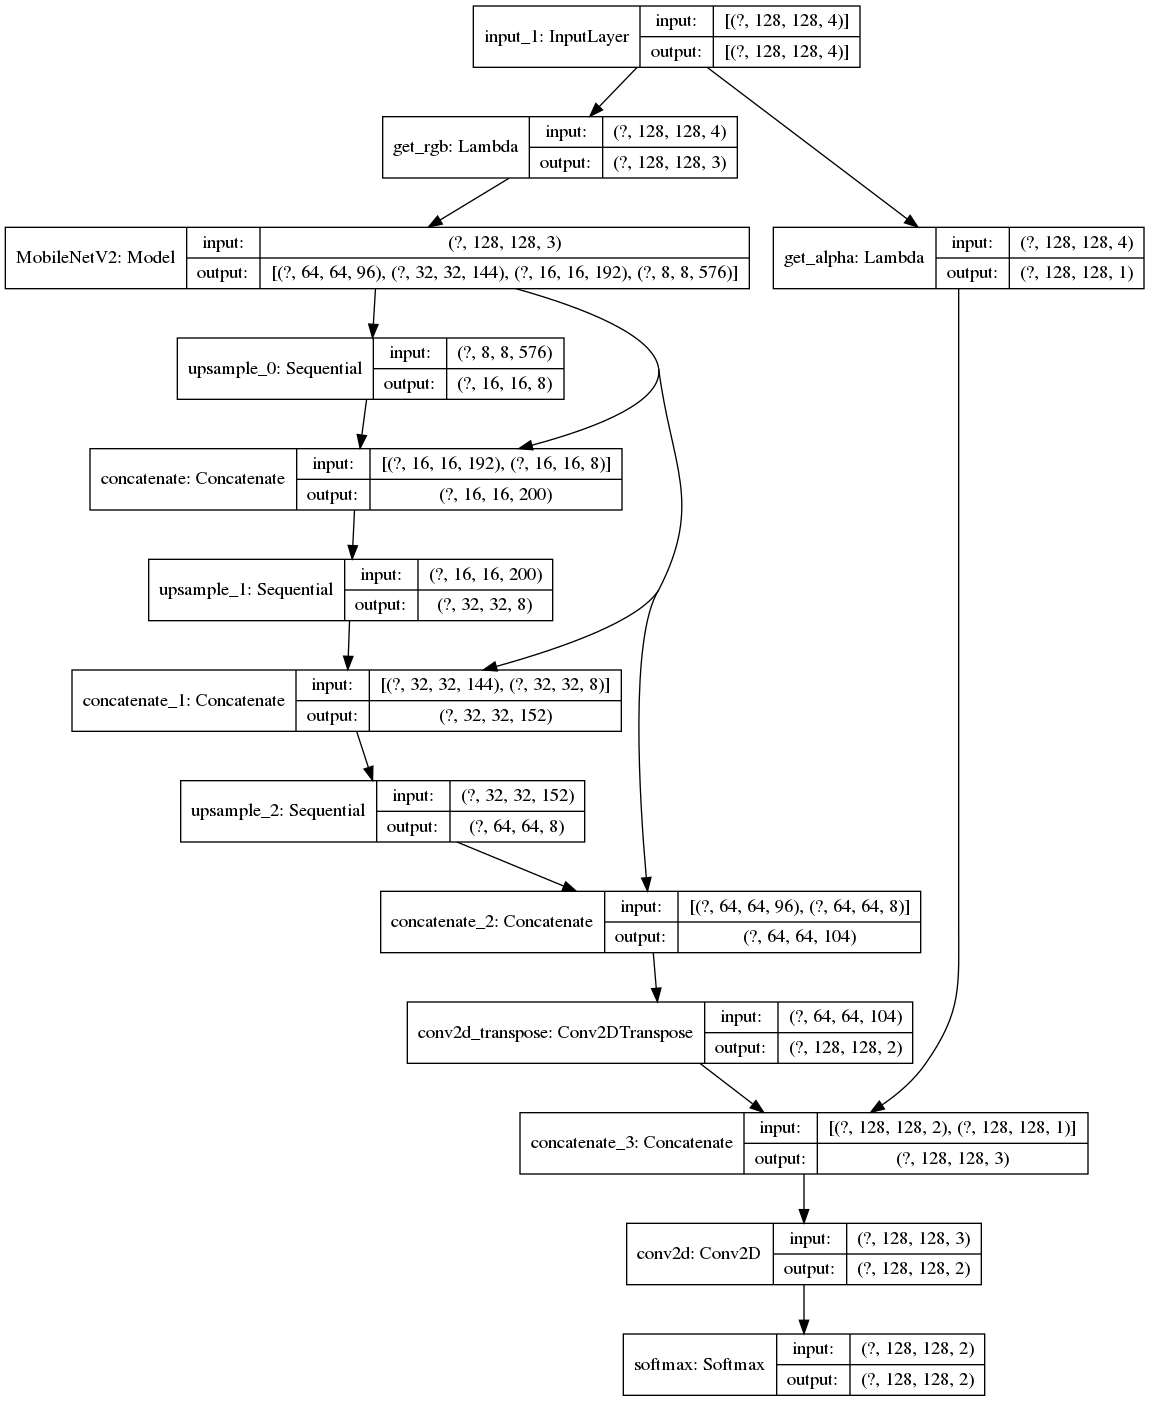
\includegraphics[width=0.9\textwidth]{images/full_model}
        \caption{Neural net architecture on top of MobileNetV2.}
        \label{f:model}
    \end{figure}

\end{document}
